\documentclass{article}
\linespread{1.3}
\usepackage[margin=50pt]{geometry}
\usepackage{amsmath, amsthm, amssymb, amsthm, tikz, fancyhdr, graphicx}
\pagestyle{fancy}
\renewcommand{\headrulewidth}{0pt}
\newcommand{\changefont}{\fontsize{15}{15}\selectfont}

\fancypagestyle{firstpageheader}
{
  \fancyhead[R]{\changefont Michael Huang \\ CFRM 420 \\ Homework 3}
}

\begin{document}

\thispagestyle{firstpageheader}

\section*{1.}
{\Large 

% \begin{verbatim}
%   Text enclosed inside \texttt{verbatim}
%   environment 
%   is printed directly 
%   and all \LaTeX{} commands are ignored.
% \end{verbatim}

% \framebox[1.1\width]{\textbf{answer}}

\subsection*{(a)}

We perform this in R using the \texttt{plot} function.

\begin{figure}[h]
  \centering
  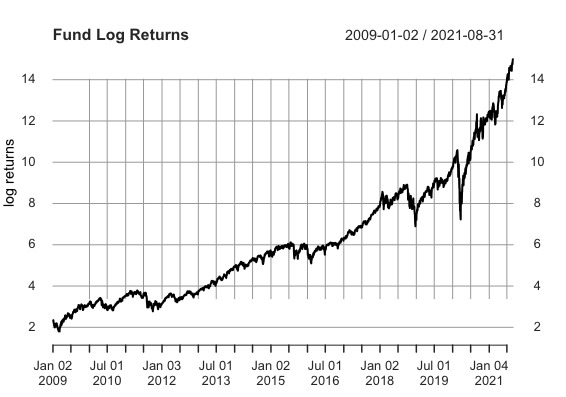
\includegraphics[width=500pt]{hw3_1a.png}}
\end{figure}

\subsection*{(b)}

We calculate these using the \texttt{mean}, \texttt{var}, \texttt{skewness} and \texttt{kurtosis}  functions (with the latter adjusted by +3, since it calculates the excess kurtosis): \\
Sample mean: \framebox[1.1\width]{\textbf{0.01320093}} \\ 
Sample variance: \framebox[1.1\width]{\textbf{0.002066732}} \\ 
Sample skewness: \framebox[1.1\width]{\textbf{-0.3651695}} \\ 
Sample kurtosis: \framebox[1.1\width]{\textbf{3.643343}}

\subsection*{(c)}

We take the volatility using the standard deviation, so we use the function \texttt{sd} to determine the volatility of the 3 assets; we take the expected returns by taking the mean, so we use the function \texttt{mean}. We get the following results: \\
Bond: 0.001756121 log returns, 0.004133538 volatility \\
Fund: 0.01320093 log returns, 0.04546132 volatility \\
S\&P 500: 0.011261 log returns 0.04137414 volatility \\ \\ 
From doing this comparison, we see that \framebox[1.1\width]{\textbf{it is not the case}} that assets with higher expected return have higher volatility. In fact, the lowest volatility asset, the bond, has the highest expected log return.

\subsection*{(d)}

We perform said functions in R, and \texttt{plot} as follows. We fit a normal distribution by taking the mean and variance of the distribution and fit as follows. \\

\begin{figure}[h!]
  \centering
  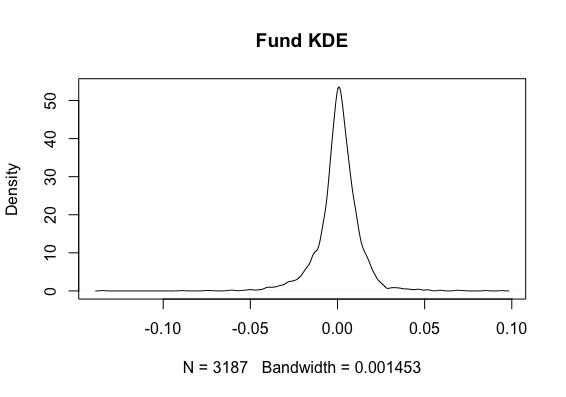
\includegraphics[width=400pt]{hw3_1d_kde.png}}
\end{figure}

\begin{figure}[h!]
  \centering
  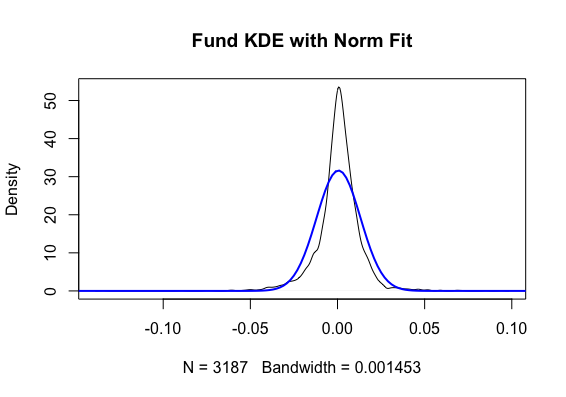
\includegraphics[width=400pt]{hw3_1d_kde_norm.png}}
\end{figure}

\subsection*{(e)}

We can compute the 1\% sample quantile of the daily log returns by using the \texttt{quantile} function, resulting in a value of \framebox[1.1\width]{\textbf{-0.03774583}}. If we were to calculate the 99\% value at risk based on the quantile of the daily log returns rather than the fitted normal distribution, this would be a better fit because as we can see in 1(d), the fitted normal distribution is not a great fit for the actual returns.

\newpage

}

\section*{2.}
{\Large

\subsection*{(a)}

The QQ plot is similar to that of a heavy-tailed distribution.

\begin{figure}[h!]
  \centering
  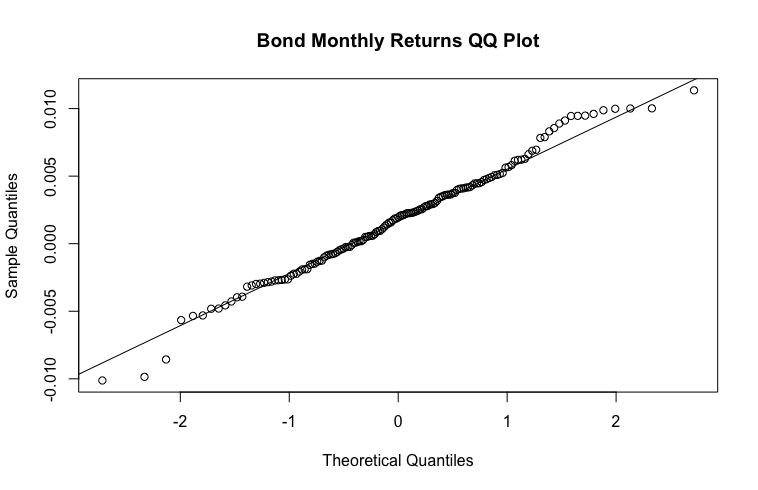
\includegraphics[width=500pt]{hw3_2a.png}}
\end{figure}

\subsection*{(b)}

We find the 25\% and 75\% sample quantiles using the \texttt{quantile} function, finding these values to be -0.004354415 and 0.006505337. We also know that the standard quantile function tells us that the values at 0.25 and 0.75 are -0.6744898 and 0.6744898. Doing some math, we find the slope to be \\
$m = \frac{0.006505337 - -0.004354415}{0.6744898 - -0.6744898} = \frac{0.010859752}{1.3489796} = 0.0080503456$ \\
and using some algebra to solve for the intercept: \\ 
$0.006505337 = 0.0080503456 \cdot 0.6744898 + b$ \\
$b = 0.006505337 - 0.00542987599$ \\ 
$b = 0.00107546101$ \\ \\ 
So our line has \framebox[1.1\width]{\textbf{slope 0.0080503456 and intercept of 0.00107546101.}}

\subsection*{(c)}

If the normal QQ plot of some sample of observations were to lie on the line described in (b), the sample distribution would be the \framebox[1.1\width]{\textbf{normal distribution.}}

}

\end{document}